\chapter{Conclusion}
The end of three years of Ph.D research is surely a significant moment. I started my Ph.D. without being sure of what the world of research was like and whether I would have been able to do a good Ph.D or not. Happily, after all this experience I can be very satisfied of what I have achieved and learned.
This thesis is the result of three years where I studied and worked on amazing topics that are one of the most important of the current decade and, presumably, of the next ones. In particular, having the feeling of being part of the huge community of researchers aiming to the progress of such a revolutionary scientific topic, represented for me a very significant achievement. Moreover, considering that I had the possibility to participate to top conferences around the world, to work in an excellent team and to be followed by a great advisor which I thank for his help, I can say this Ph.D. gave me what I was hoping for and maybe more.

\section{Recap of the thesis}
This thesis resumes the work I made during my three years of Ph.D. research about the exploitation of uncertainty in Reinforcement Learning (RL). After a first part with the introduction about general consideration on \gls{rl} and the description of preliminary concepts, the thesis is split in two parts where it is showed how uncertainty can be exploited to improve performance of state-of-the-art algorithms. In the former part, uncertainty is used to improve the estimate of the components of the update by means of the Bellman operator; in the latter part, uncertainty is used to drive exploration aiming to improve sample-efficiency of exploration policies. The exploitation of uncertainty is not a new line of research in \gls{rl}, thus my works are mainly inspired by methodologies available in literature that I considered to work out my own novel ones.

\subsection{Bellman update}
\subsubsection{What I studied}
The first work I dealt with, after the initial study of the classical literature and the state-of-the-art works, was the Double $Q$-Learning (DQL)~\cite{van2010double}. This paper addresses the problem of overestimation of the Maximum Expected Value (MEV) in the context of action-value function estimation. This happens, for instance, in $Q$-Learning (QL)~\cite{smith2006optimizer} because of the Maximum Estimator (ME) involved in the update rule via Bellman Equation (BE). The importance of \gls{dql} stands on the proposal of a variant of \gls{ql} which replaces the \gls{me} with the Double Estimator (DE) making \gls{dql} able to avoid the overestimation providing, on the contrary, an underestimation of the optimal action-values. The underestimation helps to have good learning in some problems with high stochasticity and, more in general, in problems where there is not clearly an action which is better than the others. One of the interesting aspects of the \gls{de} is that it can be used in several value-based \gls{rl} algorithms without major changes. For instance, the offline value-based algorithm of Fitted $Q$-Iteration (FQI)~\cite{ernst2005tree} can be easily modified to make it use \gls{de} resulting in what we call Double Fitted $Q$-Iteration (DDFQI) algorithm. Moreover, the ideas behind \gls{dql} have been also applied in Deep RL (DRL) with the Double Deep $Q$-Network (DDQN)~\cite{hasselt2015double}, a variant of Deep $Q$-Network (DQN)~\cite{mnih2015human} which I also considered during my research on this topic.

\subsubsection{What I did}
To address the problem of overestimation of \gls{mev}, I worked on the introduction of a novel estimator called Weighted Estimator (WE) which computes an averaged sum of action-values where the weights are the probability of each action to be the best one. I showed how the \gls{we} can be both positively or negatively biased, but its absolute bias is always less than the ones of \gls{me} and \gls{de}. I applied this estimator to \gls{ql} bringing to Weighted $Q$-Learning (WQL) which I compare to \gls{ql} and \gls{dql} in several discrete problems. Then, I proposed an extension of \gls{we} to continuous problems by means of a variant of \gls{fqi}, called Weighted Fitted $Q$-Iteration (WFQI), which uses \gls{we} and Gaussian Process (GP) regression to estimate the uncertainty of the prediction. The interesting aspect of this method is that it naturally adapts to problems with continuous actions being one of the few value-based approaches able to deal with infinite action spaces. Eventually, I studied the application of \gls{we} also in \gls{drl} introducing a variant of \gls{dqn} called Weighted Deep $Q$-Network. The adaptation of \gls{we} in \gls{dqn} is not straightforward since the computation of the uncertainty is cumbersome to obtain in neural networks. To make it practical, I took inspiration from the network architecture proposed in Bootstrapped Deep $Q$-Network (BDQN)~\cite{osband2017deep} which uses a single network which is split in multiple output resulting in an ensemble of action-value function estimates. Then, I used the estimates provided by the ensemble to work out the uncertainty to use in the computation of \gls{we}. This method is a first practical solution to use \gls{we} in \gls{dqn}, but the not satisfying preliminary results and the possibility to use different methods to compute uncertainty make this work only a first solution in this direction.

The study of the overestimation of \gls{mev} is not the only way I considered to improve the update of action-value function estimate via the \gls{be}. My second work about this introduces the $RQ$-Learning algorithm which is the result of the effort put in decomposing the \gls{be} and exploiting the uncertainty of its components, i.e. the reward and the maximum action-value. This is done considering the fact that the source of uncertainty of the two components of the \gls{be} are different and, thus, make sense to consider them separately. Together with this consideration, a different learning rate for the two components is used and adapted according to the measure of uncertainty. The method is compared with several variant of \gls{ql} (e.g. \gls{dql} and \gls{wql}) showing significant results and robustness in heterogeneous problems. I also proposed an on-policy variant of the methodology and compared it with SARSA reaching good results also in this case.

\subsection{Exploration}
\subsubsection{What I studied}
The problem of exploration in \gls{rl} is one of the most addressed in \gls{rl} literature. It deals with the purpose of the agent to cover the a significant portion of the state space of the environment in order to improve the quality of the learned policy. However, the balance between exploration and exploitation is critical in order to obtain higher performance in terms of cumulative discounted reward; therefore, an exploration policy which minimizes the number of samples needed to learn an effective exploitative policy is desirable. Among the trivial $\varepsilon$-greedy strategy which makes no use of the information acquired by the agent, the Boltzmann and mellowmax policy~\cite{asadi2016alternative} use the current estimate of the action-value function computing the next action to execute by a softmax operator.

More complex work to deal with exploration are based on the concept of Optimism in the Face of Uncertainty (OFU) which encourages the execution of actions bringing to unknown regions of the state space. This is pursued, among others, by strategies based on Thompson Sampling (TS)~\cite{thompson1933likelihood} and by the algorithms belonging to the Intrinsic Motivation (IM)~\cite{schmidhuber1991possibility} category. In exploration strategies based on TS, e.g. $Q$-value sampling~\cite{dearden1998bayesian}, the actions are sampled from the distribution modeling their probability of being the ones with the highest action-value. This has been widely studied in the context of Multi-Armed Bandit problem, but it has been proven to be an effective way to balance exploration and exploitation also in the context of \gls{rl}~\cite{auer2007logarithmic}. On the other hand the \gls{im} strategies add an intrinsic reward, which is summed to the reward returned by the environment, expressing the quality of the reached state in terms of novelty. In particular, the intrinsic reward is usually proportional to the amount of new knowledge of the state space obtained by the agent when reaching it; this way, the agent is intuitively encouraged to visit new kind of states. The challenging part of \gls{im} is to work out a measure to evaluate the novelty of a state which may significantly slow down the learning. Among others, some works address this issue proposing different ways to count the amount of similar states reached~\cite{tang2017exploration} and others introduce new measure such as the curiosity of the agent~\cite{schmidhuber1991possibility, pathak2017curiosity}.

\subsubsection{What I did}
I addressed the exploration problem analyzing both the strategies of \gls{ts} and \gls{im} that are both based on \gls{ofu}. In the first work, I introduced some algorithms to make the use of exploration strategies based on \gls{ts} practical in \gls{rl}. Indeed, several methodologies based on \gls{ts} have certainly desirable theoretical properties, but perform poorly in empirical applications. The main contribution of this work consists in the proposal of different ways of computing the uncertainty and to pursue the \gls{ofu} principle. In particular, the first way is studied for discrete problems and exploits the computation of uncertainty explained in the work about \gls{we}~\cite{deramo2016estimating} also applying statistical upper bounds to encourage exploration, while the second way is proposed as a solution for continuous high dimensional problem where the uncertainty is estimated via an ensemble of action-value function approximator as proposed in \gls{bdqn}. The different algorithms are empirically evaluated in increasingly complex problems where exploration is a critical aspect to solve them. The results highlight how they are able to reach better performance faster than other sampling strategies, thus showing the better balancing between exploration and exploitation.

The second work in this direction is more based on \gls{im} and proposes a variant of the \gls{be} called Optimistic \gls{be} (OBE). In \gls{obe}, an ensemble of action-value estimates is used to compute the update of the action-values basing on a maximum entropy principle. The entropy maximization aims to increase the action-values proportionally to their uncertainty provided by the ensemble in such a way to encourage exploration. This work is inspired by the \gls{im} literature because of the intrinsic exploration bonus assigned to the update of the action-value, but with the desirable property of not making use of any time consuming way to explicitly measuring the uncertainty. The \gls{obe} is applied in variants of \gls{ql} and \gls{dqn}, which I respectively called Optimistic \gls{ql} (OQL) and Optimistic \gls{dqn} (ODQN). This methodologies are theoretically studied, e.g. the convergence of \gls{oql} is proven, and empirically evaluated against Bootstrapped Q-Learning (BQL) and \gls{bdqn} showing better performance in the considered problems.

\subsection{Comments}
All of the described works have been done in collaboration with colleagues and/or master students working on their MSc thesis, together with the help of my advisor. While I think the works about the improvement in the Bellman update \gls{be} have been studied enough in depth, I think there is still to work on the ones about exploration. More in detail, the study of exploration strategies based on \gls{ts} brought to satisfying results both lack of theoretical guarantees to make this work interesting for publication. On the other hand, the work about the \gls{obe} is currently under review, but I think it needs to be better studied especially in its empirical evaluation.

While focusing on the problems described before, I always considered the progress in the Deep Reinforcement Learning (DRL) literature. During my Ph.D., this field has become more and more important at the point that the empirical evaluation of the novel works proposed had to be done on \gls{drl} problems, e.g. Atari games~\cite{bellemare13arcade}, to make them more appealing. In three years, I tried to work on \gls{drl} studying novel ways to improve state-of-the-art methods, e.g. smart feature extraction in \gls{dqn}, and these works brought to the publication of some MSc thesis but were not enough significant to publish at conferences. The major problems I faced in working on \gls{drl} were the very high computational demand in terms of resources and time at the point that I had to wait several days to obtain the results for a single experiment. Considering the slowness in working on \gls{drl}, I preferred to fix on practical classical \gls{rl} problems and to secondarily extend these works in \gls{drl} applications, e.g. applying \gls{we} in \gls{dqn} introducing Weighted \gls{dqn} (WDQN).

\section{Future directions}
All the works done for this thesis, the other ones I did but that are out of the focus and all the ones I studied in the literature, gave me a lot of insights on what the research in \gls{rl} is like and on the important problems that need to be addressed to improve the state-of-the-art of this field. In particular, the current effort in solving highly dimensional complex problems is resulting in outstanding performance, as in the case of chess~\cite{silver2017chess}, but is sometimes ignoring the huge increasing of computational resources to solve these problems. Indeed, typically a \gls{drl} model has an enormous amount of parameters, requires days of training time corresponding to many years of human play, often has unstable learning and most of the time the semantics of the learned representation is hard to understand at the point that it is often used in a black-box way~\cite{mnih2015human}. As a matter of fact, despite the excellent performance that a \gls{drl} model and more in general a \gls{dl} model is able to achieve, this last drawback causes serious problems of robustness of the learned representations leading to unsatisfying results. For instance, in a recent work on image classification with deep neural networks the authors show how it is possible to trick the model by means of samples specifically modified for this purpose~\cite{yuan2017adversarial}. These ``adversarial examples'' are usually samples of images slightly modified in such a way that, for instance, a single pixel is changed. The pixel is not changed randomly, on the contrary its value is smartly modified studying the gradient of the function learned by the classifier. At the end, the original sample and the adversarial one look totally the same at a human eye, but the classifier see them as completely different samples. The reasons behind this issue are multiple and the analysis of them requires a much longer discussion which is out of focus for this last section of the thesis, but substantially it can be concluded that this issue demonstrates the lack of robustness of \gls{dl} model and, more in general, the difficulty for the model to extract the real semantics of what it learns.

\begin{figure}[t]
\begin{minipage}{\textwidth}
\begin{center}
  \subfigure[Breakout\label{F:breakout_frame}]{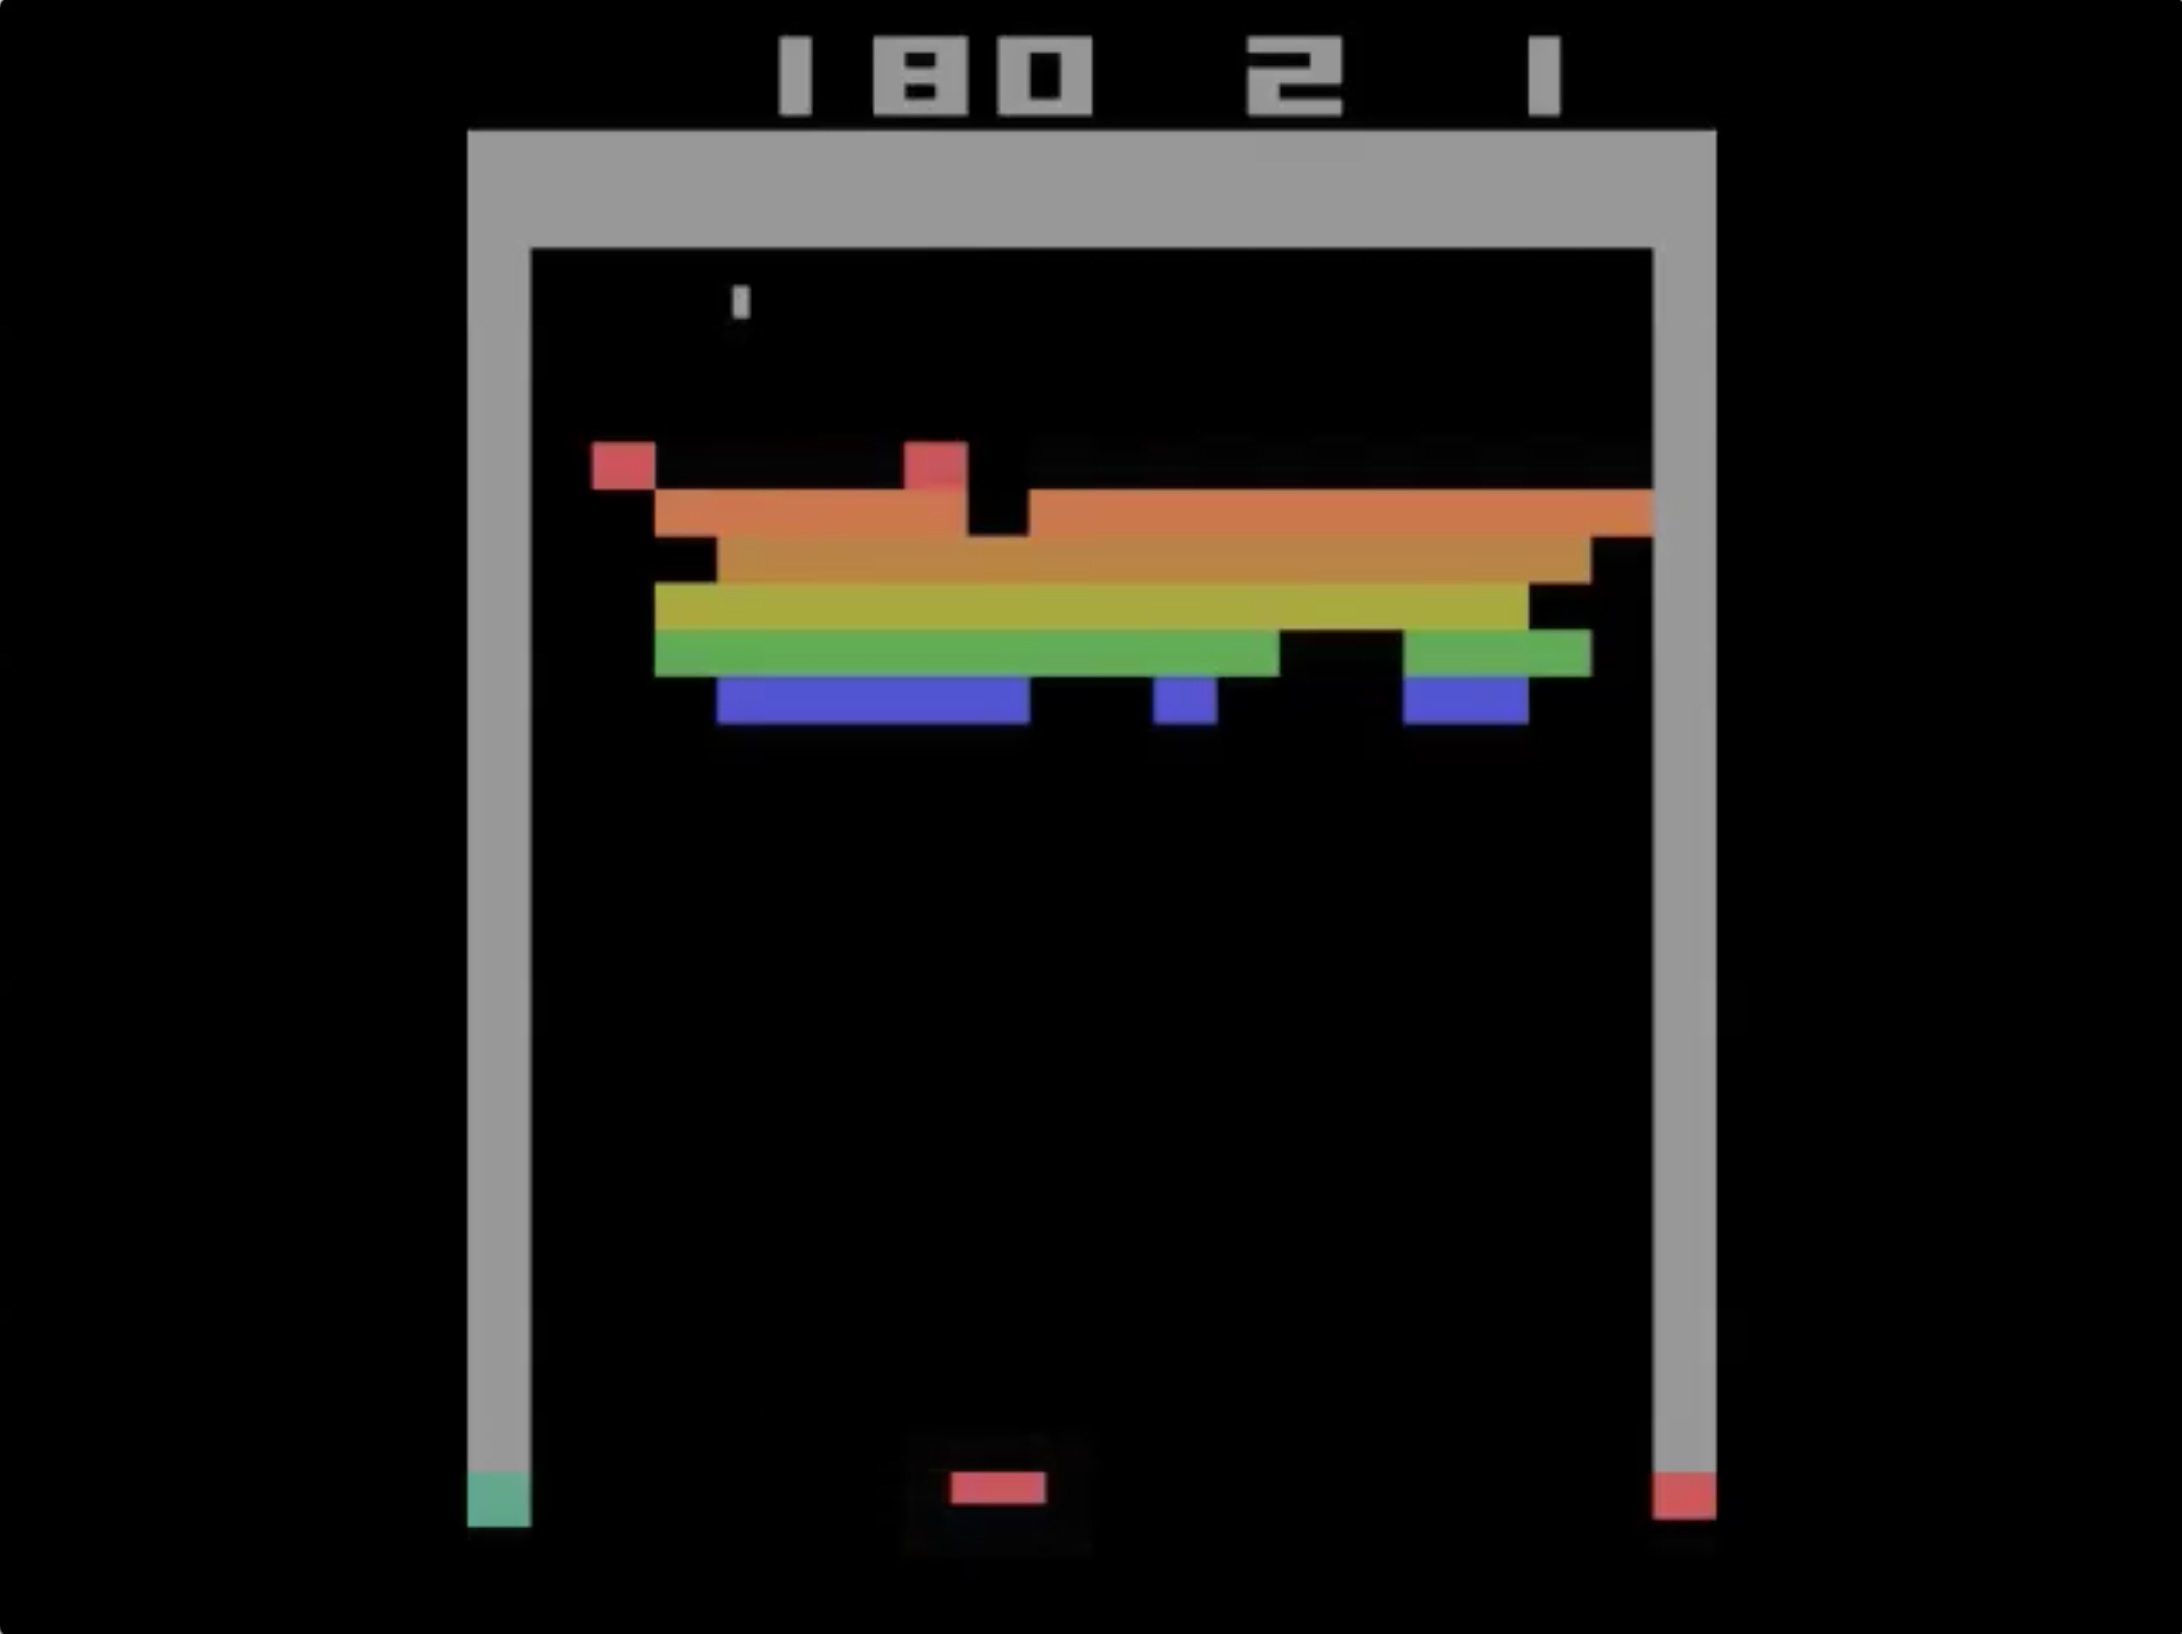
\includegraphics[scale=.01]{img/breakout.jpg}}
  \hspace{1cm}
  \subfigure[Humanoid\label{F:humanoid}]{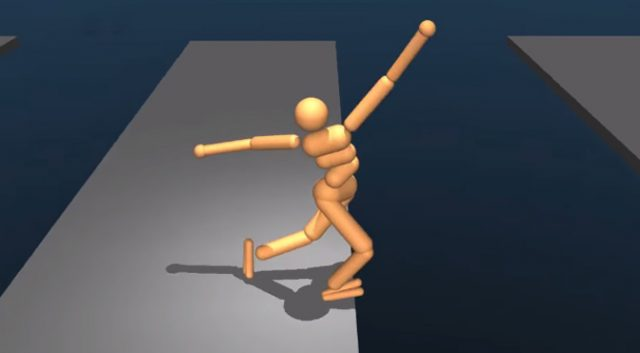
\includegraphics[scale=.3]{img/humanoid.jpg}}
\end{center}
\end{minipage}
\caption[Breakout and Humanoid problems]{Graphical rendering of Breakout and Humanoid problems.}\label{F:breakout_humanoid}
\end{figure}
Considering that the models and their fitting algorithms used in \gls{drl} are the same of \gls{dl}, it is intuitive how they can suffer of the previously described issues with impact on the quality of the learned policy. Figure~\ref{F:breakout_humanoid} show two examples of environments to highlight the problems that may arise when learning how to solve them. In particular, Figure~\ref{F:breakout_frame} refers to the Breakout game briefly described in Section~\ref{S:exploration_drl}. Recalling that in this game the purpose is to catch the ball with the platform on the bottom in order to let it bounce and hit the bricks on the wall on the top, it is intuitive how the number of features needed to solve this games are way less than all the number of pixels of the raw frame. Thus, desirably the deep $Q$-network should be able to extract only the few relevant features, such as the coordinates of the ball and the platform, in order to simplify the learning of the policy. However, usually this does not happen and the network learns a very abstract representation of the input whose semantics is practically not interpretable.
